\documentclass[a4paper,14pt]{article} % тип документа
%\documentclass[14pt]{extreport}
\usepackage{extsizes} % Возможность сделать 14-й шрифт


\usepackage{geometry} % Простой способ задавать поля
\geometry{top=25mm}
\geometry{bottom=35mm}
\geometry{left=20mm}
\geometry{right=20mm}

\setcounter{section}{0}

%%%Библиотеки
%\usepackage[warn]{mathtext}
%\usepackage[T2A]{fontenc} % кодировка
\usepackage[utf8]{inputenc} % кодировка исходного текста
\usepackage[english,russian]{babel} % локализация и переносы
\usepackage{caption}
\usepackage{listings}
\usepackage{amsmath,amsfonts,amssymb,amsthm,mathtools}
\usepackage{wasysym}
\usepackage{graphicx}%Вставка картинок правильная
\usepackage{float}%"Плавающие" картинки
\usepackage{wrapfig}%Обтекание фигур (таблиц, картинок и прочего)
\usepackage{fancyhdr} %загрузим пакет
\usepackage{lscape}
\usepackage{xcolor}
\usepackage{dsfont}
%\usepackage{indentfirst}
\usepackage[normalem]{ulem}
\usepackage{hyperref}




%%% DRAGON STUFF
\usepackage{scalerel}
\usepackage{mathtools}

\DeclareMathOperator*{\myint}{\ThisStyle{\rotatebox{25}{$\SavedStyle\!\int\!\!\!$}}}

\DeclareMathOperator*{\myoint}{\ThisStyle{\rotatebox{25}{$\SavedStyle\!\oint\!\!\!$}}}

\usepackage{scalerel}
\usepackage{graphicx}
%%% END 

%%%Конец библиотек

%%%Настройка ссылок
\hypersetup
{
colorlinks=true,
linkcolor=blue,
filecolor=magenta,
urlcolor=blue
}
%%%Конец настройки ссылок


%%%Настройка колонтитулы
	\pagestyle{fancy}
	\fancyhead{}
	\fancyhead[L]{Домашнее задание}
	\fancyhead[R]{Крейнин Матвей, группа Б05-005}
	\fancyfoot{}
    \fancyfoot[C]{\thepage}
    \fancyfoot[R]{Основные алгоритмы}
%%%конец настройки колонтитулы



\begin{document}
%%%%Начало документа%%%%

\section{Задание 10}
\subsection{Задача 1}
Воспользуемся BFS, он работает за $O(|V| + |E|)$, причем будем хранить массив размера $|V|$, в котором будет лежать инофрмация о родителе. 
Заведем счётчик $i = 0$. Посмотрим на элемент, который предшествует t, увеличим на единицу счетчик, повторяем пока в какой-то момент наш предок не будет вершиной s.
Тогда счётчик i будет показывать длину пути из s в t. 

\textbf{Корректность:} была доказана на лекции 

\textbf{Асимптотика:}
\newline
По памяти: $O(|V|)$ -- размер массива
\newline
По времени: $O(|V| + |E|)$ -- время работы BFS, $O(|V|)$ -- время обхода массива, т.е. получаем $O(|V| + |E|)$

\subsection{Задача 2}

\begin{enumerate}
	\item Корректность будет следовать из обычного алгоритма Дейкстры, т.к. без отрицательных ребер он не будет дополнительно записывать вершины в очередь,
	т.к. для вычеркнутых вершин уже будет найдено минимальное расстояние.
	\item Принцип работы будет такой же, как и у обычного, отличие будет в том, что в обычном алгоритме, если вершина обработана в очереди, то её приоритет
	-- минимальное расстояние, с ребрами отрицательной длины так не будет работать. Поэтому, если расстояние до какой-то вершины уменьшилось, то её опять надо обработать, т.к.
	расстояние дл вершин, путь которых проходит через эту вершину тоже уменьшится. Корректность, модифицированного алгоритма следует из корректности обычного алгоритма
	(если мы выкинули вершину в обычной модификации алгоритма, то мы нашли минимальное расстояние, т.к. все расстояния неотрицательные,  а в модифицированной версии, т.к. есть ребра отрицательной длины, вычеркивание вершины
	не означает, что мы нашли минимальное расстояние до этой вершины, поэтому нужно опять проверить вершины, до которых расстояние уменьшилось). С циклами отрицательной не нужно работать, т.к. алгоритм никогда не остановится,
	ходя по циклу и уменьшая расстояние до $-\inf$.
	\item Посчитаем сумму отрицательных ребер. Очевидно, что никакой путь не сможет быть меньше этой длины, т.к. в пути все ребра встречаются не больше одного раза, т.к. нет циклов отрицательной длины.
	Тогда будем проверять не стала ли длина от вершины отсчета до некторой вершины меньше, чем S, если стала, то это будет циклом.
\end{enumerate}

\subsection{Задача 3}
Алгоритм будет не корректен. Есть два пути, один длиной -2, а другой длиной -3.
\begin{center}
	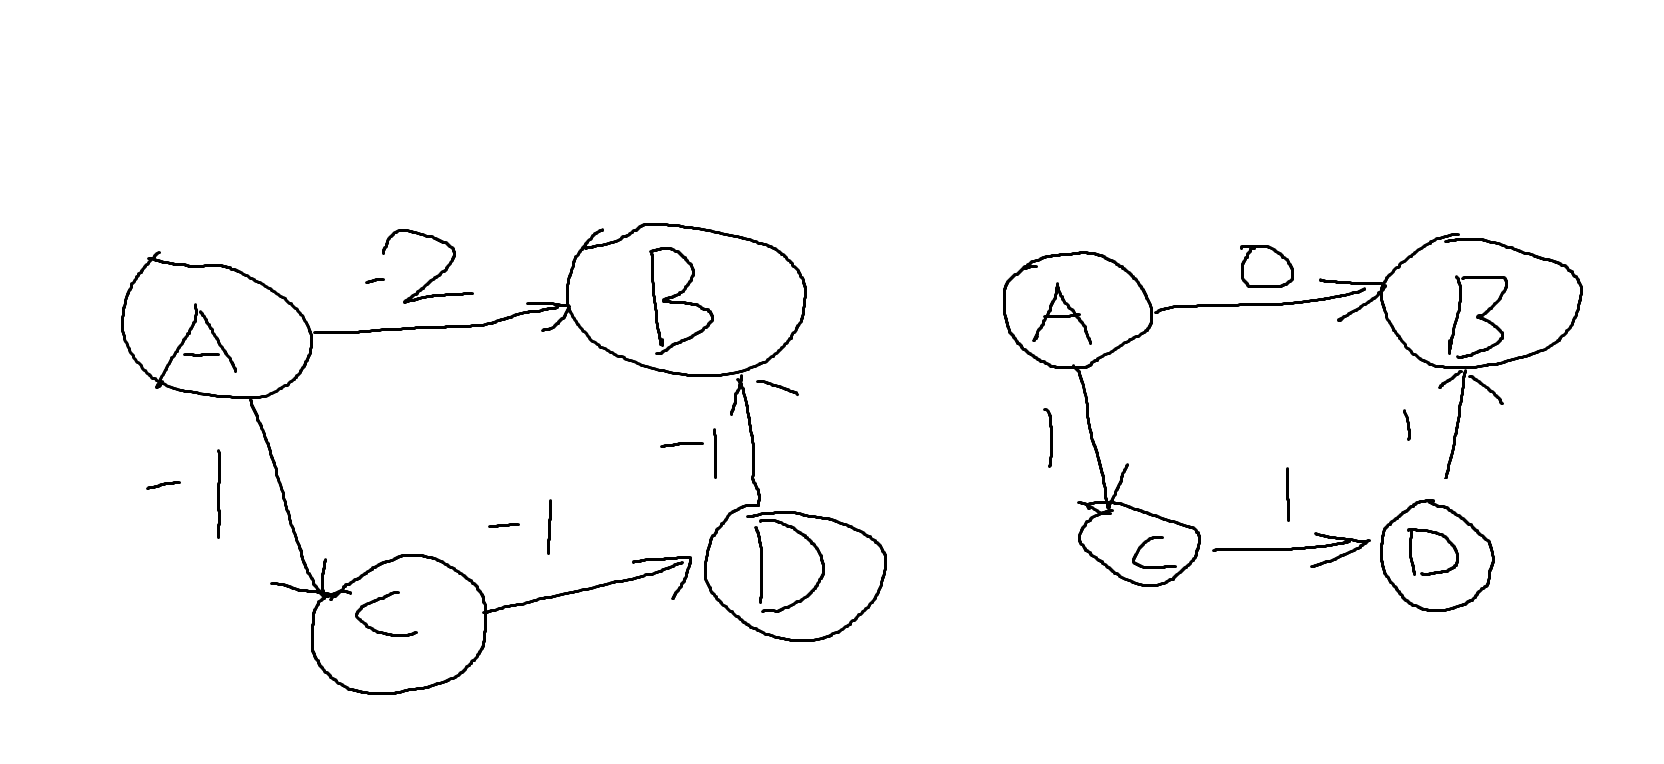
\includegraphics[scale=0.5]{01.png}
\end{center}
Видно, что после прибавления константы 2 ко всем вершинам, у нас изменится кратчайший путь.
Предложенный алгоритм не корректен.

\subsection{Задача 4}
Модифицируем BFS, добавив вторую очередь. Пусть вершина, от которой ищем расстояние будте S. Положим её в первую очередь, все соседей, расстояние до которых равно 1, положим в первую очередь, а все остальных, до которых расстояние 0, покрасим и положим во вторую очередь.
Перейдем ко второй очереди -- идем по ней до тех пор пока она не закончится, если расстояние от обрабатываемой вершины до её соседа равно нулю, то красим и записываем во вторую очередь, а если 1, то кладем в первую.
Когда вторая очередь закончится вернемся к первой и идем по ней, пока после какой-нибудь вершины вторая очередь снова станет непустой. Переключаемся на вторую очередь и идем по ней, пока она не закончится.
Таким образом получилось связать вершины, между которыми расстояние равно нулю.

\textbf{Корректность: } следует из корректности BFS.

\textbf{Асимптотика: } такая же, как $O(|V| + |E|)$, т.к. сравнения на цвет требуют $O(|V|)$, а проход по второй очереди ещё $O(|V|+|E|)$.

\subsection{Задача 5}
Будем рассматривать все пути из s в t, заметим, что после транспонирования ребер путь максимальной длины из s в t останется также максимальным путем из s в t.
Допустим, что после транспонирования получился новый путь - не обратный путю из s в t. Но тогда транспонировав обратно, он будет путем из s в t, а значит такого не может быть.
Т.е. максимальный путь из s в t -- это максимальный путь из t в s после транспонирования ребер. Используем алгоритм Беллмана-Форда -- коректность была доказана на лекции.

\textbf{Асимптотика:} для транспонирования ребер: $O(|E|)$, для поиска максимального пути $O(|V|)$, а время работы Беллмана-Форда: $O(|E|+|V|)$, т.е. $O(|E|+|V|)$.

\subsection{Задача 6}
Каждое дерево двудольно, т.е. мы можем раскрасить вершины так, чтобы концы каждого ребра были покрашены в разный цвет. Возьмем произвольную вершину за корень. Используемся BFS и вершины, находящиеся на нечетном расстояние от неё покрасим.
Они и будут образовывать максимальное назависимое множество.

\textbf{Корректность: } на каждом нечетном уровне дерева будут вершины из искомого множества, между нечетными уровнями два ребра, а посередине непокрашенная вершина, т.е. у этих двух ребер разноцветные вершины.
Если попали в лист, то тоже ничего не будет нарушено, т.к. либо он будет покрашен, а предшествующая нет, либо наоборот.

\textbf{Асимптотика:} время работы BFS: $O(|V|+|E|)$, время покраски $\Theta(\frac{|V|}{2})$, т.е. $O(|V|+|E|)$

\end{document} 
